\documentclass[11pt]{article}
\usepackage{times}
\usepackage{amssymb}
\usepackage{amsfonts}
\usepackage{amsmath}
\usepackage{braket}
\usepackage{latexsym}
\usepackage{enumerate}
\usepackage{graphicx}
\usepackage{mathtools}
\usepackage{xifthen}
\usepackage{bbold}
\usepackage{xargs}
\usepackage{url}
\usepackage{slashed}
\usepackage{hyperref}
\usepackage{adjustbox}
\usepackage{subcaption}
\usepackage{cleveref}
\usepackage{svg}
\usepackage{wrapfig}

\usepackage{listings}
  \lstset{
    language=Lisp,
    basicstyle=\ttfamily\scriptsize,
    breaklines=true,
    columns=fullflexible,
    keepspaces=true,
    showstringspaces=false
  }

\hypersetup{colorlinks=true,linkcolor=blue,urlcolor=blue}

\usepackage{tikz}
\usepackage[compat=1.1.0]{tikz-feynman}

\setlength{\oddsidemargin}{.25in}
\setlength{\evensidemargin}{.25in}
\setlength{\textwidth}{6in}
\setlength{\topmargin}{-0.4in}
\setlength{\textheight}{8.5in}

\newcommand{\handout}[6]{
   \renewcommand{\thepage}{#1-\arabic{page}}
   \noindent
   \begin{center}
   \framebox{
      \vbox{
    \hbox to 5.78in { {\bf {#6}} \hfill Due: #2 }
       \vspace{4mm}
       \hbox to 5.78in { {\Large \hfill #1: #5  \hfill} }
       \vspace{2mm}
       \hbox to 5.78in { {\it Name: #3 \hfill Collaborators: #4} }
      }
   }
   \end{center}
   \vspace*{0mm}
}

\DeclareMathOperator{\tr}{tr}
\newcommand{\dd}[2]{\frac{\partial #1}{\partial #2}}
\newcommand{\ddn}[3]{\frac{\partial^#3 #1}{\partial #2^#3}}
\renewcommand{\d}{\delta}
\newcommand{\D}{\Delta}
\newcommand{\Lx}{\hat{L}_x}
\newcommand{\Ly}{\hat{L}_y}
\newcommand{\Lz}{\hat{L}_z}
\newcommand{\Lp}{\hat{L}_{+}}
\newcommand{\Lm}{\hat{L}_{-}}
\newcommand{\Lpm}{\hat{L}_{\pm}}
\renewcommand{\L}{\hat{L}}
\renewcommand{\l}{\lambda}
\newcommand{\el}{\ell}
\newcommand{\px}{\hat{p}_x}
\newcommand{\py}{\hat{p}_y}
\newcommand{\pz}{\hat{p}_z}
\newcommand{\p}{\hat{p}}
\newcommand{\td}{\dot{t}}
\newcommand{\tdd}{\ddot{t}}
\newcommand{\rd}{\dot{r}}
\newcommand{\rdd}{\ddot{r}}
\newcommand{\xd}{\dot{x}}
\newcommand{\xdd}{\ddot{x}}
\newcommand{\vd}{\dot{v}}
\newcommand{\vdd}{\ddot{v}}
\newcommand{\yd}{\dot{y}}
\newcommand{\ydd}{\ddot{y}}
\newcommand{\zd}{\dot{z}}
\newcommand{\zdd}{\ddot{z}}
\renewcommand{\i}{\hat{i}}
\renewcommand{\j}{\hat{j}}
\renewcommand{\k}{\hat{k}}
\newcommand{\x}{\hat{x}}
\newcommand{\y}{\hat{y}}
\newcommand{\z}{\hat{z}}
\renewcommand{\r}{\hat{r}}
\newcommand{\rh}{\hat{r}}
\newcommand{\expect}[1]{\left\langle #1 \right\rangle}
\renewcommand{\a}{\alpha}
\newcommand{\adag}{a^\dagger}
\newcommand{\ad}{a^\dagger}
\newcommand{\hb}{\hbar}
\newcommand{\h}{\hbar}
\renewcommand{\b}{\beta}
\newcommand{\e}{\epsilon}
\newcommand{\s}{\sigma}
\renewcommand{\t}{\tau}
\renewcommand{\td}{\dot t}
\newcommand{\g}{\gamma}
\newcommand{\w}{\omega}
\renewcommand{\k}{\kappa}
\renewcommand{\u}{\mu}
\renewcommand{\v}{\nu}
\newcommand{\kphi}{\ensuremath{\ket{\phi}}}
\newcommand{\kpsi}{\ensuremath{\ket{\psi}}}
\newcommand{\bphi}{\ensuremath{\bra{\phi}}}
\newcommand{\bpsi}{\ensuremath{\bra{\psi}}}
\newcommand{\Z}{\mathbb Z}
\newcommand{\R}{\mathbb R}
\newcommand{\C}{\mathbb C}
\newcommand{\cross}{\times}
\newcommand{\Tau}{\tau}
\newcommand{\dH}{\d H}
\newcommand{\del}{\vec \nabla}
\newcommand{\curl}{\del \cross}
\let\oldexp\exp
\renewcommand{\dag}[1]{ #1^\dagger }
\renewcommand{\exp}[1]{\oldexp \left( #1 \right) }
\renewcommand{\bf}[1]{\textbf{#1}}
\newcommand{\eqn}[1]{\begin{align*} #1 \end{align*}}
\newcommand{\pmat}[1]{\begin{pmatrix} #1 \end{pmatrix}}
\newcommand{\ans}[1]{ \Aboxed{#1} }
\newcommand{\ansa}[1]{ \eqn{ \Aboxed{#1} } }
\newcommand{\textans}[1]{
\noindent\vspace*{3mm}\\\vspace*{3mm}\fbox{\begin{minipage}{\linewidth}{#1}\end{minipage}}
}
\newcommand{\tensor}{ \otimes }
\newcommand{\emf}{ \mathcal{e} }
\newcommand{\1}{ \mathbb{1} }
\newcommand{\sech}{ \text{sech} }
\DeclarePairedDelimiter\abs{\lvert}{\rvert}%
\DeclarePairedDelimiter\norm{\lVert}{\rVert}%
\makeatletter
\let\oldabs\abs
\def\abs{\@ifstar{\oldabs}{\oldabs*}}
%
\let\oldnorm\norm
\def\norm{\@ifstar{\oldnorm}{\oldnorm*}}
\makeatother

\usepackage{titlesec}
\usepackage{lipsum}

% \titleformat{\section}[runin]%shape
%           {\Large\bfseries}%format
%           {Problem \thesection}%label
%           {0pt}%sep
%           {: }%before
%           []%after

\newcommand{\problem}[3]{
\ifthenelse{\equal{#1}{}}{}{\setcounter{section}{#1-1}}
\section{#2} \hfill \ifthenelse{\equal{#3}{}}{}{ \small [#3] }\\
}


% \titleformat{\subsection}[runin]%shape
%           {\large \bfseries}%format
%           {Problem \thesubsection}%label
%           {0pt}%sep
%           {: }%before
%           []%after

\newcommand{\subproblem}[3]{
\ifthenelse{\equal{#1}{}}{}{\setcounter{subsection}{#1-1}}
\subsection{#2} \hfill \ifthenelse{\equal{#3}{}}{}{ \small [#3] }\\
}



\newcommand{\ppart}[2]{
\noindent\vspace*{3mm}\\ {\large #1} \ifthenelse{\equal{#2}{}}{}{ [{\bfseries #2}] }
}

\newcommand{\inst}[1]{
\vspace{3mm}
\item[] \hspace{-3mm} { #1 }
\vspace{4mm}
}

\usepackage[letterpaper, margin=1in]{geometry}
\begin{document}

\handout{Mini-Paper 3}{\textbf{November 9, 2026}}{Don't forget to add your name}
{List all sources used}{Abelian Sandpile Model}{CS598APE}

\vspace*{1em}
\noindent The final mini-paper this semester is to analyze and improve the end to end performance of a 2D finite Abelian Sandpile. The scope of this homework is designed to be smaller than the other 2 homeworks, in order to let you focus more on your projects.

For this project, you will work \textbf{individually}, and the grading will be based on your report~(\cref{subsec:report}) and your artifact evaluation~(\cref{subsec:artifact}). You will also peer review the reports and artifacts of others.

You are welcome to use any source of inspiration or tool to create your optimizations, subject to the \href{https://prontolab.github.io/598APE/about/}{course policy on the website}. These may include new code/changes to code and the use of different tools to generate or change code. You are welcome to also try more advanced techniques that do not fall into this category (e.g. specific hardware). For precise details, check \cref{subsec:artifact}. 

\section{Accessing Course Infrastructure}
You are welcome to use any hardware of your choosing to test and perform optimizations, assuming that the optimizations you write can be replicated by others. This does not mean that others need to replicate your exact performance results (e.g. exactly $12\%$ boost by doing X), but that the optimization you write generally results in an improvement and does not rely on non-standard hardware features. If you want to use your own machine for setup and optimization, you are responsible for ensuring the requisite requirements are available.

We have given students access to \href{http://prontolab.github.io/598APE/about/#compute-infrastructure}{UIUC teaching VMs}. You may use them for completing the homeworks and project.

\section{Abelian Sandpile Model}

An abelian sandpile of size $N \times N$ is a grid containing the number 0,1,2
and 3 (representing the number of grains of sand). Adding two sandpiles works by
first adding element by element, and then \textit{toppling} any element that
goes over 3. A toppling removes four grains from that cell and sends one to
each of its four direct neighbors. Grains that fall off the grid disappear.

The order in which you topple doesn't matter, since the end result always
remains the same (hence the term \textbf{abelian}). We write
$\operatorname{stab}(S)$ for the stable sandpile obtained by toppling until
every cell has at most three grains, and define sandpile addition by
$A \oplus B = \operatorname{stab}(A+B)$, where $+$ is elementwise addition.
For example, add the following two $3 \times 3$ sandpiles and stabilize:
\begin{align*}
  \begin{pmatrix} 3 & 3 & 3 \\ 3 & 3 & 3 \\ 3 & 3 & 3 \end{pmatrix}
  +
  \begin{pmatrix} 1 & 2 & 1 \\ 2 & 1 & 2 \\ 1 & 2 & 1 \end{pmatrix}
  &=
  \begin{pmatrix} 4 & 5 & 4 \\ 5 & 4 & 5 \\ 4 & 5 & 4 \end{pmatrix}
  \xrightarrow{\text{stabilize}}
  \begin{pmatrix} 2 & 1 & 2 \\ 1 & 0 & 1 \\ 2 & 1 & 2 \end{pmatrix}.
\end{align*}
The arrow summarizes a sequence of topplings.

We are interested in the \textit{recurrent} sandpiles: the stable configurations
that can be obtained by adding grains to the all-3s grid and stabilizing.
These form a group $G$ under $\oplus$. 

Any group $G$ (it can be numbers, vectors, or in this case the recurrent
sandpiles) has a special element called the identity element. The identity
element $e_N$ has the following property -- for any element $x \in G$ 

\begin{align*}
  x \oplus e_N = x
\end{align*}

In the case of the integer set $\mathbb{Z}$, we have $\oplus = + $ (just addition), and
the identity element is just the number \textbf{0}.

Similarly, \textit{recurrent sandpiles} form a group, which has a unique
identity. For the $3\times 3$ case, this identity sandpile is just
\begin{align*}
  e_3 &= \begin{pmatrix} 2 & 1 & 2 \\ 1 & 0 & 1 \\ 2 & 1 & 2 \end{pmatrix}.
\end{align*}
For example, adding $e_3$ to the all-2s sandpile leaves it unchanged after
stabilization:
\begin{align*}
  \begin{pmatrix} 2 & 2 & 2 \\ 2 & 2 & 2 \\ 2 & 2 & 2 \end{pmatrix}
  + e_3
  &=
  \begin{pmatrix} 4 & 3 & 4 \\ 3 & 2 & 3 \\ 4 & 3 & 4 \end{pmatrix}
  \longrightarrow
  \begin{pmatrix} 0 & 5 & 0 \\ 5 & 2 & 5 \\ 0 & 5 & 0 \end{pmatrix}
  \\
  &\longrightarrow
  \begin{pmatrix} 2 & 1 & 2 \\ 1 & 6 & 1 \\ 2 & 1 & 2 \end{pmatrix}
  \longrightarrow
  \begin{pmatrix} 2 & 2 & 2 \\ 2 & 2 & 2 \\ 2 & 2 & 2 \end{pmatrix}.
\end{align*}

The arrows topple the four corners, the four edge centers, and finally the
center. 

Identity sandpiles show some interesting symmetric structure when you scale $N$
upto very high values. For example, this is the identity sandpile for a $401
\times 401$ grid of values. Black denotes $0$ grains, Blue denotes $1$ grain,
Pink denotes $2$ grains and Gold denotes $3$ grains.

\begin{center}
  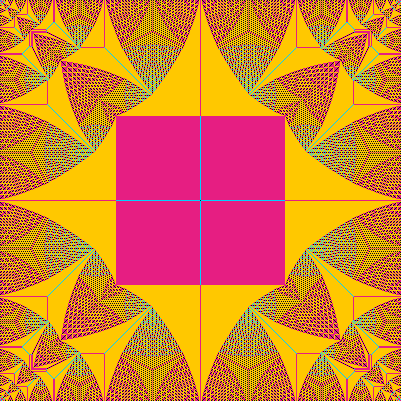
\includegraphics[width=0.45\linewidth]{id401_square.png}
\end{center}

We can also change the shape of the underlying grid to be something other than a
square. We still see the appearance of structure (e.g a triangular grid). 

\begin{center}
  
\includegraphics[width=0.45\linewidth]{id401_triangle.png}
\end{center}


% \begin{figure}
%   \centering
%   % \captionsetup{labelformat=empty}
%   \includesvg[width=0.5\textwidth]{Ray_trace_diagram.svg}
%   \caption{High level view of a ray tracer in action.}
%   \label{img:raytrace}
% \end{figure}

% \begin{center}
% \includesvg[width=0.5\textwidth]{Ray_trace_diagram.svg}    
% \end{center}
\subsection{Where Is the Code?}
The application code for this project is \href{https://github.com/PRONTOLab/598APE-HW3-F26}{available on GitHub}. Fork this code, but please keep your code and optimizations in private (and not public) repositories. 

The README.md contains more information about the layout of the symbolic regression code and how to execute it. 

\subsection{What is your Task?}
For this homework, you will be expected to find the identity sandpile for a 1001
$\times$ 1001 Pacman-esq grid. It looks like this 

\begin{center}
  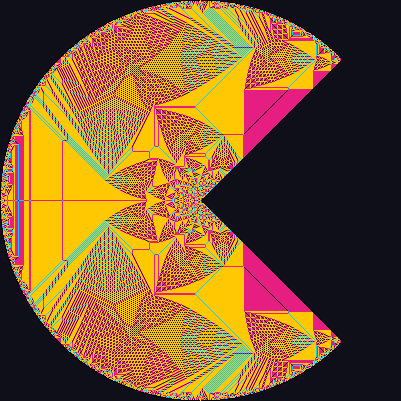
\includegraphics[width=0.45\linewidth]{id401_pacman.png}
\end{center}

\section{How to Tackle this Homework}
\begin{enumerate}
    \item Create a private fork of the homework repository on GitHub. Instructions on how to do that are in \href{https://gist.github.com/vimarsh6739/d920781b429f1ef8ec559e62aecd0e12}{this GitHub gist}. 
    \item Look at the code, see where you can make some obvious improvements. Profile, identify bottlenecks, and optimize them. Keep doing this again and again. \href{https://martin.leyrer.priv.at/y2022/m09/premature_optimisation.html}{Don't prematurely optimize}. 
    \item Use \href{https://www.brendangregg.com/perf.html}{\texttt{perf}} to identify performance hotspots in your code. One super easy way to get started is to use \texttt{perf} to produce a \href{https://www.brendangregg.com/FlameGraphs/cpuflamegraphs.html}{flamegraph}, and see the busiest functions in your code.
    \item Use debuggers like \href{https://sourceware.org/gdb/}{\texttt{gdb}} or \href{https://rr-project.org/}{\texttt{rr}} to assist you with debugging. Ensure that your programs are safe from memory leaks using tools like \texttt{valgrind}.  
    \item Implement one optimization at a time. This helps in reasoning about your optimizations, and reproducing the effect of a specific optimization if needed. 
    % \item We encourage you to go wild with ideas to improve performance(for your own pleasure). Here are some approaches which the TA thinks might be fun to try out:
    % \begin{itemize}
    %     \item Switch to LLVM and use \href{https://github.com/google/souper}{souper} or \href{https://github.com/minotaur-toolkit/minotaur}{minotaur} to optimize your code using a SMT solver. 
    %     \item Try adding RTX support(Nvidia GPUs)
    %     \item If there are any stencil-like computations, maybe use \href{https://github.com/halide/Halide}{Halide} with it's autoscheduler. 
    % \end{itemize}
    \item Document your approach in the report. Make sure your code is reproducible (the whole point of \texttt{Docker} is to avoid the \textit{oh but it runs on my computer...} )
    \item Review \& run the code your peers write!
\end{enumerate}

\section{What to Hand In}
\subsection{Report}
\label{subsec:report}
Your report should be about (and no more than) $3$ pages long(excluding references). Use the \href{https://www.overleaf.com/latex/templates/association-for-computing-machinery-acm-sigplan-proceedings-template/rfvsrhgmghtc}{ACM Sigplan Template} (follow the formatting in \texttt{sample-sigplan.tex}). It should include:
\begin{enumerate}
    \item A \textbf{brief description} of your optimizations. This can include optimizations which helped performance, optimizations which did not help performance, or potential optimizations you did not implement and why (for example as profiling indicated it not to be helpful). Describe what kind of optimization you tried (e.g. algorithmic, data-structure, parallelism, caching, work-reduction, etc).
    \item \textbf{Specify the assumptions} which an optimization relies on, and the scope in which your optimization applies. For example, one could hardcode the application to directly output the desired image (perhaps conditional on the exact input specification) -- but this would only provide a speedup for that scene at that resolution.
    \item \textbf{Include graphs} to indicate performance improvements/slowdowns (if any). Remember, the goal here is to not just get blind speedups, but also attempt to investigate why we are getting those speedups (or perhaps why we are not). %We encourage you to show the use of profiling information(if any) you used to 
    \item A brief \textbf{introspection} section for your optimizations: Performance engineering involves coming up with ideas that can improve performance, and profiling/deciding which ones will be impactful in practice. Sometimes you can do something but speedup up a function $100\times$ that represents $<1\%$ of runtime won't change much. Similarly, sometimes you need to do prerequisite optimizations before the fruit of a bigger optimization can apply (e.g. rewrite a datastructure to be a linear scan is required before caching can be improved).
\end{enumerate}

\subsection{Artifact}
\label{subsec:artifact}
You will be expected to submit an artifact, which will be independently evaluated by random team. To ensure the ease of reproducibility, the artifact should be a well documented \href{https://git-scm.com/}{git} repo which should have at-least the following things in it's README.md

\begin{enumerate}
    \item \textbf{All the tools needed to construct a binary from your source code}. We recommend modifying \texttt{docker/Dockerfile} and specifying the packages needed to install/build your tools. 
    \item \textbf{Instructions on how to build and run} your code. This includes how to run and benchmark your baseline code, and verify that your optimizations hold water. Remember, part of your grade depends on whether your peers are able to replicate the results stated in your paper. 
    \item \textbf{List your optimizations, and what commands, flags, or earlier git commits} are needed to evaluate their effectiveness.
\end{enumerate}

\paragraph{Custom Hardware} You are welcome to also try more advanced optimizations that require specific hardware to run -- for example GPU tensor cores, RTX, DLSS, \href{https://www.intel.com/content/www/us/en/docs/intrinsics-guide/index.html#techs=AVX_512}{Intel AVX-512} or \href{https://developer.arm.com/architectures/instruction-sets/intrinsics/#f:@navigationhierarchiessimdisa=[Neon]&f:@navigationhierarchiesinstructiongroup=[Vector%20arithmetic]}{Arm NEON} intrinsics(for the M1 Mac folks...). 

However, \textbf{in this case you must submit two artifacts}: one artifact which can be run by anyone with a standard Unix machine (like the provided course VMs or Docker files), and a second artifact detailing optimizations based on non-replicable setups. We recommend using separate git branches or commit hashes to easily distinguish both artifacts.

\section{How to Submit?}

You will be using HotCRP to submit and peer-review your reports. We will open up the submission link as soon as the deadline nears.  As for the code, it is sufficient to provide a link to the github repo you will be using for writing the code. 

% \section{Grading Rubric}
% % to be filled in...

% \section{Some Tutorials}
% Please refer to \href{https://gist.github.com/vimarsh6739/d920781b429f1ef8ec559e62aecd0e12}{this gist} on a tutorial to help you out with the following aspects of the homework:
% \begin{itemize}
%     \item Forking a private copy of a public repo. 
%     \item How to use \texttt{perf}
% \end{itemize}

% The \href{https://github.com/PRONTOLab/598APE-HW1/tree/main?tab=readme-ov-file#docker}{README.md on the project page} has enough information on how to build and run your own \texttt{Dockerfile} if you need more pre-existing software. 

\clearpage
%   \appendix
%
% {\Large\bfseries Appendix\par}
%
%
%   \section{Reconstruction Source Code}
%   \label{app:reconstruct-source}
%
%   The following Racket program was generated by genetic programming
%   for the \texttt{silk-wave} benchmark. Each RGB channel averages
%   three learned symbolic expressions. Executing the program renders
%   the reconstructed PNG image.
%
%   The source code and inputs for both benchmarks are available in the
%   \href{https://github.com/PRONTOLab/598APE-HW2}{GitHub repository}.
%
%   \subsection{Silk Wave}
%   % TODO: Replace the previous homework's listing with the sandpile source.
%   % \lstinputlisting{silk-ref.rkt}
\end{document}

